\section{Lección \#1 - Conozcamos al triángulo rectángulo}
Cualquier estudiante de enseñanza media sabe que se trata de un triángulo que tiene un ángulo con amplitud $90\degree$. Sin embargo no muchos saben la cantidad de relaciones que se generan en ese polígono. Dediquemos entonces un tiempo al estudio de este triángulo tan ``generoso''.

\begin{multicols}{2}
    \begin{tikzpicture}[
      my angle/.style={
        every pic quotes/.append style={text=black},
        draw=white,
        angle radius=1cm,
      }]
      \coordinate [label=left:] (B) at (-2,-1.5);
      \coordinate [label=right:] (A) at (2,-1.5);
      \coordinate [label=above:] (C) at (-2,1.5);
      \draw (B) -- node[left] {$a$} (C) -- node[above] {$c$} (A) -- node[below] {$b$} (B);
      \draw (B) +(.25,0) |- +(0,.25);
      \pic [my angle, "$\alpha$"] {angle=C--A--B};
      \pic [my angle, "$\beta$"] {angle=B--C--A};
    \end{tikzpicture}
\columnbreak\\
1) \textbf{Teorema de Pitágoras}\\
\[c^2 = a^2 + b^2\]\\
2) \textbf{Razones Trigonométricas}
\begin{align*}
\sen\alpha &= \dfrac{a}{c}\\
\cos\alpha &= \dfrac{b}{c}\\
\tan\alpha &= \dfrac{a}{b}\\
\sen\alpha &= \cos\beta
\end{align*}
\end{multicols}

- Vea que basta conocer la longitud de dos lados o la amplitud de uno de los ángulos agudos y la longitud de uno de los tres lados para determinar el resto de los cinco elementos del triángulo.

\begin{multicols}{2}
    \begin{tikzpicture}[
      my angle/.style={
        every pic quotes/.append style={text=black},
        draw=white,
        angle radius=1cm,
      }]
     \coordinate [label=left:] (B) at (-2,-1.5);
      \coordinate [label=right:] (A) at (2,-1.5);
      \coordinate [label=above:] (C) at (-2,1.5);
      \coordinate [label=above:] (H) at (-0.56,0.42);
      
      \coordinate (F) at (-0.76,0.57);
      \coordinate (J) at (-0.91,0.37);
      \coordinate (K) at (-0.51,0.07);
      \coordinate (G) at (-0.36,0.27);
      
      \draw (F) -- (J);
      \draw (J) -- (K);
      \draw (K) -- (G);
      
      \draw (B) -- node[left] {$a$} (C);
      \draw (B) -- node[below] {$b$} (A);
      \draw (C) -- node[above] {$p$} (H);
      \draw (A) -- node[above] {$q$} (H);
      \draw (B) -- node[above] {$h$} (H);
    
      \pic [my angle, "$\alpha$"] {angle=C--A--B};
      \pic [my angle, "$\beta$"] {angle=B--C--A};
      \pic [my angle, "$\omega$"] {angle=H--B--C};
      \pic [my angle, "$\sigma$"] {angle=A--B--H};
    \end{tikzpicture}
\columnbreak\\
3) \textbf{Grupo de Teoremas de Pitágoras}
\vspace*{-0.1cm}
\begin{align*}
3.1)\hspace{1cm}h^2 &= p \cdot q\\
3.2)\hspace{1cm}a^2 &= c \cdot p\\
b^2 &= c \cdot q\\
3.3)\hspace{1cm}c^2 &= a^2 + b^2
\end{align*}
\end{multicols}

- Es suficiente conocer la longitud de dos de los seis segmentos determinados, o uno de ellos y uno de los cuatro ángulos determinados para calcular el valor del resto de los diez elementos

\subsubsection{Demostración de 3)}

Sean $\triangle_1$, $\triangle_2$ y $\triangle_3$ de lados $(a,h,p)$, $(a,b,c)$ y $(b,h,q)$ tenemos:
\begin{equation*}
 \left.\begin{aligned}
        \triangle_1 \sim \triangle_2 &: \dfrac{a}{c}=\dfrac{h}{b}=\dfrac{p}{a} \Longrightarrow a^2 = c \cdot p\\
    \triangle_2 \sim \triangle_3 &: \dfrac{b}{c}=\dfrac{h}{a}=\dfrac{q}{b} \Longrightarrow b^2 = c \cdot q
       \end{aligned}
 \right\}
 \qquad \textbf{3.2) Teorema de los catetos}
\end{equation*}
\hspace{1.3cm}$\triangle_1 \sim \triangle_3: \dfrac{a}{b}=\dfrac{h}{q}=\dfrac{p}{h} \Longrightarrow h^2 = p \cdot q$\hspace{0.1cm} \qquad \textbf{3.1) Teorema de la altura}\\

Sumando las dos ecuaciones obtenidas en $3.2$:
\begin{align*}
    a^2 + b^2 &= c \cdot p + c \cdot q\\
              &= c (p + q)\\
              &= c \cdot c\\
              &= c^2 \qquad\qquad\qquad\qquad\qquad\qquad\qquad\textbf{3.3) Teorema de Pitágoras}
\end{align*}

Vea además que el área del triángulo podemos expresarla como:
\begin{center}
$A = \dfrac{ab}{2}$ y $A = \dfrac{ch}{2}$ $\Longrightarrow$ $\dfrac{ab}{c} = h$    
\end{center}

Vea también que $\sigma = \beta$ y $\omega = \alpha$ por ser ángulos agudos con lados respectivamente perpendiculares

\begin{multicols}{2}
4)\vspace*{-0.5cm}\\
\hspace*{0.9cm}
    \begin{tikzpicture}
      \coordinate [label=left:$C$] (B) at (-2,-1.5);
      \coordinate [label=right:$B$] (A) at (2,-1.5);
      \coordinate [label=above:$A$] (C) at (-2,1.5);
      \coordinate [label=above:$M$] (H) at (0,0);
    %   \draw (B) -- node[left] {$a$} (C) -- node[above] {$c$} (A) -- node[below] {$b$} (B);
      \draw (B) -- node[left] {} (C);
      \draw (B) -- node[below] {} (A);
      \draw (C) -- node[above] {} (H);
      \draw (A) -- node[above] {} (H);
      \draw (B) -- node[above] {} (H);
    %   \draw (H) +(-.25,0) |- +(0,.25);
    \end{tikzpicture}
\columnbreak\\

Sea $M$ punto medio de $\overline{AB}$

$\Longrightarrow \overline{AM} = \overline{MB} = \overline{CM}$
\begin{center}
\textbf{Teorema de la mediana de la\\ hipotenusa}
\end{center}
\end{multicols} 

\subsubsection{Demostración}
\begin{itemize}
    \item[$\cdot\hspace{0.05cm}\text{-})$] Sea $\overline{MH}\perp\overline{CB}$ en $H \Longrightarrow \overline{MH}$ es la paralela media de $\overline{AC}$\\
\hspace*{2cm}$\therefore \overline{MH}$ es altura y mediana de $\overline{BC}$ en $\triangle CMB$\\
\hspace*{2cm}o sea, $\triangle CMB$ es isósceles de base $\overline{CB}$, etc...

    \item[$\cdot\hspace{0.05cm}\text{-})$] Sea $D$ un punto de la prolongación de $\overline{CM}$; $\overline{CM} =\overline{MD} \Longrightarrow ACBD$ es paralelogramo-rectángulo y $\overline{AM}=\overline{MB}=\overline{CM}=\overline{MD}$ por propiedades de un triángulo

    \item[$\cdot\hspace{0.05cm}\text{-})$] $M$ es circuncentro del $\triangle ABC \Longrightarrow \overline{AM}=\overline{MB}=\overline{MC}=$ radio de la circunferencia de centro $M$ que pasa por $A$, $B$ y $C$ (recíproco del teorema de Tales)
\end{itemize}


\noindent5) En todo triángulo rectángulo con un ángulo agudo de $30\degree$ tenemos:
\begin{itemize}
    \item[i)]El cateto opuesto al ángulo de $30\degree$ mide la longitud de la hipotenusa dividida por dos ($a = c \div 2$) 
    \item[ii)]El cateto adyacente al ángulo de $30\degree$ mide $\sqrt{3}$ veces la longitud del cateto opuesto al ángulo de $30\degree$ ($b = \sqrt{3}a$)
\end{itemize}

\subsubsection{Demostración}
\begin{multicols}{2}
    \begin{tikzpicture}[
      my angle/.style={
        every pic quotes/.append style={text=black},
        draw=white,
        angle radius=1cm
      }]
      \coordinate [label=left:] (A) at (0,4);
      \coordinate [label=left:] (B) at (0,0);
      \coordinate [label=above:] (C) at (3.46,2);
      \coordinate [label=left:] (M) at (0,2);
      \draw[dashed] (B) -- node[left] {$a$} (M);
      \draw (M) -- node[left] {$a$} (A);
      \draw (M) -- node[above] {$b$} (C);
      \draw (A) -- node[above] {$c$} (C);
      \draw[dashed] (C) -- node[below] {$c$} (B);
      \draw (M) +(.25,0) |- +(0,.25);
      \draw (M) +(.25,0) |- +(0,-0.25);
      \pic [my angle, "$60\degree$"scale=0.8] {angle=M--A--C};
      \pic [my angle, "$60\degree$"scale=0.8] {angle=C--B--M};
      \pic [my angle, "$30\degree$"scale=0.8] {angle=A--C--M};
      \pic [my angle, "$30\degree$"scale=0.8] {angle=M--C--B};
    \end{tikzpicture}
\columnbreak\\
\noindent Reflejando el triángulo dado de lados $(a,b,c)$ sobre el cateto $b$ obtengo un triángulo equilátero\\
$\Longrightarrow$ i) $a = \dfrac{c}{2}$\\
\hspace*{0.7cm}ii) $b = \sqrt{3}a$ (por Teo. de Pitágoras)\\

\noindent nota: De aquí se obtienen las razones trigonométricas de los ángulos $30\degree$ y $60\degree$
\end{multicols} 


\noindent6) En todo triángulo rectángulo e isósceles tenemos:
\begin{itemize}
    \item[] La longitud de la hipotenusa es igual a $\sqrt{2}$ veces la longitud de los catetos ($c = \sqrt{2}s$) Esto es resultado de aplicar teorema de Pitágoras con $a=b$
    \item[] nota: de aquí se obtienen las razones trigonométricas del ángulo de $45\degree$
\end{itemize}


\noindent\textbf{*} 7) En todo triángulo rectángulo, la suma de la longitud del inradio y el circunradio es igual a la media aritmética de los catetos.

\subsubsection{Demostración}
\begin{multicols}{2}
    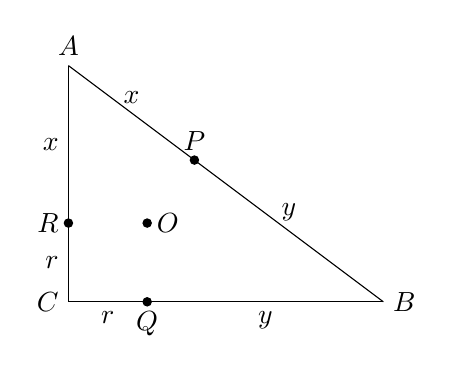
\begin{tikzpicture}
        \coordinate [label=left:$C$] (C) at (-2,-1.5);
        \coordinate [label=right:$B$] (B) at (2,-1.5);
        \coordinate [label=above:$A$] (A) at (-2,1.5);
        \coordinate [label=above:$P$] (P) at (-0.4,0.3);
        \coordinate [label=below:$Q$] (Q) at (-1,-1.5);
        \coordinate [label=left:$R$] (R) at (-2,-0.5);
        \coordinate [label=right:$O$] (O) at (-1,-0.5);
            
        \draw (A) -- node[left] {$x$} (R);
        \draw (R) -- node[left] {$r$} (C);
        \draw (C) -- node[below] {$r$} (Q);
        \draw (Q) -- node[below] {$y$} (B);
        \draw (B) -- node[above] {$y$} (P);
        \draw (P) -- node[above] {$x$} (A);
              
        \filldraw (O) circle[radius=1.5pt];
        \filldraw (P) circle[radius=1.5pt];
        \filldraw (Q) circle[radius=1.5pt];
        \filldraw (R) circle[radius=1.5pt];
      
    \end{tikzpicture}
\columnbreak\\
\noindent Sean $P$, $Q$, $R$ puntos de tangencia del incírculo del $\triangle ABC$ con los lados $\overline{AB}$, $\overline{BC}$, $\overline{CA}$, tenemos:
\begin{itemize}
    \item[] $\overline{AR}=\overline{AP}=x$
    \item[] $\overline{RC}=\overline{CQ}=r$ (inradio)
    \item[] $\overline{PB}=\overline{QB}=y$
\end{itemize}
\end{multicols} 

\begin{equation*}
    \begin{aligned}
        \Longrightarrow a &= \overline{CQ} + \overline{QB} = r + y\\
        b &= \overline{AR} + \overline{RC} = x + r\\
        c &= \overline{AP} + \overline{PB} = x + y = \text{diámetro del circuncírculo}\\
        \Longrightarrow a +b &= r + y + x + r = 2R + 2r\\
        \Longrightarrow r + R &= \dfrac{a+b}{2} 
    \end{aligned}
\end{equation*}

8) , 9). 10), ... pueden ser sugerencias de los lectores a este humilde trabajo.


\section{Lección \#2 - Rectas y Puntos Notables}
lección 2

\section{Lección \#3 - Circunferencia y Cuadrilátero}

\section{Lección \#4 - Otros Teoremas}

\section{Lección \#5}

\section{Lección \#6}

\section{Lección \#7 - Continuación}

\section{Lección \#8 - Continuación}

\section{Lección \#9 - Continuación}

\section{Lección \#10 - Trigonometría}

\section{Lección \#11 - Continuación}

\section{Lección \#12 - Sustituciones}

\section{Lección \#13 - Continuación}

\section{Lección \#14 - Teorema de Vieta}

\section{Lección \#15 - Continuación}

\section{Lección \#16 - Continuación}

\section{Lección \#17 - Los números primos}

\section{Lección \#18 - Continuación}

\section{Lección \#19 - Ecuaciones en enteros}

\section{Lección \#20 - Continuación}

\section{Lección \#21 - Continuación}

\section{Lección \#22 - Problemas de Teoría de números}

\section{Lección \#23 - Continuación}

\section{Lección \#24 - Continuación}

\section{Lección \#25 - Continuación}

\section{Lección \#26 - Continuación}